\section{Introduction}
\indent Current measurements on the determination of the transition form factor have been performed in the space-like region ($\mathrm{q}^2<0$) in collider experiments. However, due to experimental limitations (e.g. $\pi^{\pm}$ contamination in lepton sample, low branching fractions, external conversion contamination), transition form factors in the time-like region ($\mathrm{q}^2>0$) have not yet been precisely determined. Recent measurements of the time-like transition form factor for $\etaP \to e^+e^- \gamma$ have been performed by the BESIII collaboration with insufficient statistical precision to distinguish between different theoretical approaches. 
\subsection{Motivation}
While very successful in many aspects, the Standard Model of particle physics (SM)
leaves a few important questions unanswered. On the one hand, it predicts
an amount of matter that survived annihilation after the Big Bang that is many orders
of magnitude less compared to what is observed. In addition, since masses
of matter particles appear as parameters in the SM, it does not provide any understanding
why the values of these masses span so many orders of magnitude.
In addition, within the SM, phenomena like Dark Matter and Dark Energy can not be explained.
These and some more 
issues suggest that there must be physics beyond the SM, and many experiments
world-wide hunt for signals of it. 

One of the currently most promising candidates to provide a signal for physics beyond the SM
is the muon anomaly. It is a low-energy observable, which
can be both measured and computed to high precision~\cite{Jegerlehner:2009ry,Blum:2013xva}.
``The anomaly is defined by $a_\mu = (g-2)/2$, where the Land\`e g-factor is the proportionality constant that relates the spin to the magnetic moment.
 For the muon, as well as for the electron and tauon,
  the anomaly $a$ differs slightly from zero (of order $10^{-3}$)
  because of radiative corrections. In the Standard Model, contributions to the anomaly come from virtual `loops' containing photons and the known massive particles.''~\cite{miller} 
 The present experimental value $a_\mu^{\rm EXP}= 1\ 165\ 920\ 89 (63)\times 10^{-11}$
comes from the BNL E821 experiment~\cite{Bennett:2006fi}.  This value
deviates from the SM prediction by about 3 standard
deviations $\Delta a_\mu^{({\rm EXP-SM})}= (287\pm 80)\times 10^{-11}$~\cite{Davier:2010nc} 
or $= (261\pm 78)\times 10^{-11}$~\cite{Hagiwara:2011af}, depending on how the leading-order
hadronic contributions are evaluated.  While this discrepancy
is not large enough to claim a failure of the SM, it is currently the largest
deviation of a SM prediction from an experimental observable. This
alone justifies the efforts currently taken to improve both the theoretical as well as the experimental value.
New measurements are planned within the next four years at 
Fermilab/USA~\cite{Grange:2015fou} and also at JPARC/Japan~\cite{Saito:2012zz}. The goal
of the measurements is to reduce the uncertainty by a factor of four. 
In parallel the SM prediction needs to be improved in accuracy 
by at least a factor of two to establish a deviation from the SM for the first time.


The largest uncertainty of the SM prediction comes from
the hadronic quantum corrections~\cite{Jegerlehner:2009ry}.
At the level of accuracy that is relevant at the moment the hadronic
contributions can be split up into the hadronic vacuum polarization
(HVP), displayed on the left-hand side of figure \ref{fig:gm2}, and the
hadronic light-by-light scattering (HLbL), displayed in the middle of
Fig.~\ref{fig:gm2}. The most important contribution to the latter
comes from the pseudoscalar pole contributions, displayed explicitly on the right-hand 
side of Fig.~\ref{fig:gm2}. For those one expects that the contribution
should be largely saturated by the lightest exchange particles, namely the 
$\pi^0$, the $\eta$ and the $\eta'$. 
%
\begin{figure}[!h]
	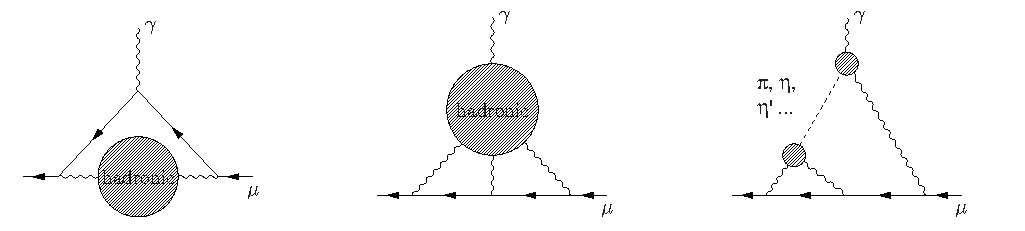
\includegraphics[keepaspectratio,width=1.\textwidth]{figures/intro/hadronicgm2.pdf}
	\caption{Hadronic contributions to $a_\mu$: hadronic vacuum polarization (left diagram), 
		hadronic light-by-light scattering (middle), pion-pole contribution to hadronic light-by-light scattering (right). Full lines with an arrow denote muons, wiggly lines photons, the dashed line a pseudo-scalar meson and shaded blobs a non-pointlike hadronic substructure. The upper blob in the right diagram corresponds to Fig.~\ref{fig:piz.dalitz}, while the lower blob corresponds to the double Dalitz decay. 
	}
	\label{fig:gm2}
\end{figure}

Concerning the SM prediction for $a_\mu$ HLbL is suppressed relative to HVP by one power of the electromagnetic
fine structure constant~\cite{Jegerlehner:2009ry,Bijnens:2007pz}.  
Unfortunately at present it is not possible to straightforwardly 
calculate the contributions shown in Fig.~\ref{fig:gm2} 
from first principles analogously to, e.g., the QED corrections, since
both processes concern low-energy corrections,
i.e.\ non-perturbative physics. Thus the prime candidate for a SM
calculation of hadronic corrections seems to be lattice QCD~\cite{Gattringer:2010zz}. 
However, it is not expected that lattice QCD
results for HPV will reach the required accuracy in the foreseeable future.
For the HLbL only preliminary lattice-QCD calculations have been reported~\cite{Blum:2014oka}.  
In view of the challenges to determine
a four-point function that includes in addition disconnected diagrams
it is not clear yet when a profound lattice calculation with
controlled uncertainties and a reliable error estimate will be
available.

Fortunately there is an alternative way to quantify hadronic corrections. It requires both
theoretical as well as experimental efforts:
Dispersion theory provides a link between particular hadronic cross sections
and $a_\mu$---for a discussion of the HVP in this context see Ref.~\cite{Jegerlehner:2009ry}, while 
for HLbL we refer to Refs.~\cite{Colangelo:2014dfa,Pauk:2014rfa,Colangelo:2014pva,Colangelo:2015ama}.  
In particular for the latter contribution it allows one to calculate from the transition
form factors of the kind $\pi^0$, $\eta$, $\eta'\to \gamma^*\gamma^*$ 
the corresponding piece for the meson pole contribution as displayed in the
right most diagram of Fig.~\ref{fig:gm2}.
The measurements proposed here provide important information towards
the necessary input needed for the evaluation of the HLbL contribution, since
$\eta'\to \gamma^*\gamma$ gives the single off-shell form factor of the $\eta'$
and $\phi\to \eta\gamma$ additionally provides information on the isoscalar
piece of $\eta\to \gamma^*\gamma$ in a different kinematic regime.
Additional information on the  $\eta$ and
$\eta'$ form factors can be found from the dispersive methods outlined in
Refs.~\cite{Adlarson:2011xb,Stollenwerk:2011zz,Hanhart:2013vba,Kubis:2015sga,Xiao:2015uva}.
It  appears to be realistic that this joined effort of theory and experiment
will provide the improvements necessary to push the SM calculation towards
the required accuracy. For the $\etaP$ pole contribution a precision of 15\% on the HLbL correction are feasible.~\cite{Nyffeler}.

\subsection{History}
\indent In the year 1951, Richard Dalitz published a letter~\cite{Dalitz} in which he calculated the rate for the \pizT  decaying into an electron-positron pair (dilepton) and a photon, \pizDal. The calculation assumed that the decay proceeded through a two–photon decay in which one of the photons was virtual and converted into an electron-positron pair.  This kind of reaction is now known as Dalitz decay. The experimental evidence of this decay process was first observed in emulsion plates exposed to the Chicago cyclotron in 1952~\cite{Lord} and a number of experiments performed over the next ten years verified Dalitz’s hypothesis that the \pizDal \ decay resulted from emission of a virtual photon~\cite{Samios,Lindenfeld,Sargent}. A few years later N. Kroll and W. Wada calculated the framework for Dalitz decays within the QED framework~\cite{KrollWada}, and extended the framework to double Dalitz Decays, in which the \pizT decays into two electron-positron pairs via emission of two virtual photons. \\
\indent Throughout the following years, much work was done to extend the framework of Dalitz decays to heavier mesons, such as \etaT, \omT, \etaTP, and \phiT. With numerous experimental data taken, it was shown that the shape of the dilepton mass spectrum deviated from the QED predictions. Such deviations are attributed to the meson not being point-like, as calculated in QED, but instead to the internal structure of the meson. The virtual photon, that decayed into a dilepton pair, has the ability to probe the structure of meson because, like its on-shell counterpart, emission of a  virtual photon is radiation, which decouples from any strong interaction within the meson when the meson transitions into its decay. Therefore, the information of the transition is encoded into the virtual photon, known as the Transition Form Factor (TFF), and can be characterized as $\left| F(q^2)\right|$, where $q^2$ is the square of the invariant mass of the lepton pair. The transition form factor can be determined by comparing QED predictions to the experimentally measured rate. Previous experimental results will be shown in Sec.~\ref{sec:current}.

\subsection{Proposal}
\indent In this proposal we present an experiment to study the $\etaP$ meson which decays via Dalitz decay, \etaPDal. The \etaTP \ is produced via electro-production, $ep \rightarrow ep\etaP$ in Hall B, using the CLAS12 detector. 
The CLAS12 detector will be used to identify and measure the $e^+e^-$ decay products by means of the High Threshold Cherenkov Counter (HTCC), Pre-Calorimeter (PCAL) and Electromagnetic Calorimeter (EC). The combination of HTCC+PCAL+EC can provide a rejection factor for single $e^\pm/\pi^\pm$ of up to $10^5$ for momenta less than 4.9~GeV/c with $\approx$ 100\% efficiency. For dileptons ($e^+e^-$ pairs), this rejection factor will be $\approx 10^{10}$, which enables dilepton studies for branching ratios $\approx 10^{-7}$. Precise determination of momenta and angles of the $e^+e^-$ decay products are the key features available to CLAS12. The momentum and angle of final state photons will be determined in CLAS12 by using the PCAL and EC. Consequently, the photon in the process $\eta^{\prime} \rightarrow e^+e^- \gamma$ will be detected. 
%The superior $e^+e^-$/$\pi^+\pi^-$ discrimination of the CLAS12 detector will give access to measurements for which  $e^+e^-$/$\pi^+\pi^-$ branching ratios of $\gtrsim 10^{10}$ are achievable.
This proposal is organized as follows. In Section~\ref{sec:kinematics}, an explanation of the kinematics of the decay processes will be given as well as kinematics of main competing backgrounds. In Section~\ref{sec:current}, we summarize the current knowledge of Dalitz decays and transition form factors, challenges in dilepton signal quality. Also a brief discussion on past CLAS analysis will be given, along with and how the CLAS12 detector can surpass the current challenges in measuring a TFF, for $\etaP$, of low statistical error. In Section~\ref{sec:measurement} a description of the analysis techniques that have been used and will be used in a CLAS12 measurement. Also in Section~\ref{sec:measurement}, an explanation of the Monte-Carlo simulations that were performed to extract the acceptances will be given as well as a calculation of expected yield and a validity check on the expected yield from previous CLAS analyses. In Section~\ref{sec:beamrequest} we present the beam time request.



